\documentclass[11pt, a4paper, USenglish]{article} % change ``USenglish'' to ``norsk'' if applicable.

\usepackage{kyblab} % Contains all included packages. See kyblab.sty.
\addbibresource{bibliography.bib} % Makes the bibliography file available to biblatex.


\begin{document}

% Titlepage
\title{Detection Project Report}
\author{Group 61\\Student Kenny Hoang Nguyen 478374\\Student Martin Lund Haug xxxxx\\}
\date{April, 2020}
\begin{titlepage}
    \maketitle
    \begin{figure}
    \centering
    \includegraphics[width=0.5\textwidth]{figures/logontnu_eng.pdf}\\
    \end{figure}
    \thispagestyle{empty}
\end{titlepage}

% Abstract
\newpage
\begin{abstract}

A short summary using about half a page about:
\begin{enumerate}[i]
    \item The course/project
    \item the results
    \item conclusion
\end{enumerate}
\end{abstract}
\thispagestyle{empty} % Avoid page numbering on the summary page.

% TOC
\newpage
\tableofcontents
\thispagestyle{empty} % Avoid page numbering on the table of contents.

% Main content
\newpage
\setcounter{page}{1}
\section{Introduction}\label{sec:intro}
Detection problems occurs in many places in everyday life, in your computer you have electrical signals which the CPU has to detect as 1 or 0, or in other words a current is present or not. Another example is in air defense where the military has radars to detect if there is an hostile air action present or not. In this project we are going to look at a cognitive radio system with primary users (PU) and secondary users (SU), where the SUs are going to detect if there are PUs in the network so that they can decide if they can utilize the frequency spectrum without interfering with the quality of service (QoS) of the PUs.\\
This problem where the SUs use the frequency spectrum in an opportunistic manner whenever there are IDLE PUs is interesting since in wireless communication systems, spectrums are a scarce resource that service providers pay a substantial amount of money to the government in order to license the spectrum. This cost is covered by the customers in their monthly mobile subscription cost. Paying customers demands a certain QoS, which in the mentioned case is the PUs, and any interference appearing on the communication channel should be kept at a minimum to deliver the promised QoS.\\
This project starts by introducing the theoretical background necessary to understand and solve this problem in section \ref{sec:theory}. Then the tasks that needs to be solved for this problem is in section \ref{sec:task} followed by the implementation and results in section \ref{sec:results} then finally it is all wrapped up in \ref{sec:conclusion}.\\

Here we should write about
\begin{enumerate}[i]
	\item The goals/motivation of the course/project.
	\item Why is your task of general interest to society? etc\dots
	\item How the report is organized
	\begin{itemize}
		\item In chapter x the theory is described
		\item in chapter y the implementation is described
		\item \dots
		\item and finally the conclusion is given in chapter z
	\end{itemize}
\end{enumerate}

\section{Theory}\label{sec:theory}
\subsection{Gaussian Distribution}
The gaussian distribution or the normal distribution is an important distribution that is often used in natural and social sciences for real-valued random variables when their distributions are not known. The importance of this distribution comes from the central limit theorem, that states for any under some conditions the average of many (enough) observations of a random variable with finite mean and variance converges to a normal distribution even if the random variable comes from another distribution.\cite{WikipediaGaussian}. The most important thing here is that the probability density function of a normal distribution with mean $\mu$ and variance $\sigma^2$ is
\begin{equation}
	f(x) = \frac{1}{\sqrt{2\pi\sigma^2}}e^{-\frac{1}{2}(\frac{x-\mu}{\sigma})^2}
\end{equation}
which gives the probability to obtain any value $x\in\mathbb{R}$ from this distribution.\\
In this particular project we use the complex gaussian distribution which for our random variables has the probability density function
\begin{equation}
	f(x) = \frac{1}{\pi\sigma^2}e^{-\frac{1}{\sigma^2}|x-\mu|^2}
\end{equation}
Which in this case take in any value $x\in\mathbb{C}$.
\subsection{$\chi^2$ distribution}
In this project the $\chi^2$ distribution is also an important distribution that is going to be used. The reason for this is because it has a more approachable point distribution function that is easier to handle when finding the cumulative distribution of a square normal distribution. The most important property of the $\chi^2$ is that it is the distribution of a sum of the squares of a $k$ independent standard normal variables with $k$ degrees of freedom.\cite{WikipediaChi}
\subsection{Estimators}
When we with probable cause can say something about the distribution that the random variables are sampled from, but not their mean and/or variance, we can estimate these distributions properties. Assumed that the random variables are sampled independent from the same identical distribution (iid), then the mean can be estimated with the average of the samples, which is unbiased.
\begin{align}
	\hat{\mu} & = \mathbb{E}\{\frac{1}{N}\sum_{n=0}^{N-1}x\}\nonumber\\
	& = \frac{1}{N}\sum_{n=0}^{N-1}\mathbb{E}\{x\}\nonumber\\
	& = \frac{1}{N}\sum_{n=0}^{N-1}\mu\nonumber\\
	& = \mu\label{eq:mu_est}
\end{align}
Meaning that the expected value of the mean of the samples will, with the number of samples taken, converge to the actual expected value of the distribution.\\
This is also the case if there are samples of the variance of the data available
\begin{align}
	\hat{\sigma^2} & = \mathbb{E}\{\frac{1}{N}\sum_{n=0}^{N-1}\sigma^2\}\nonumber\\
	& = \frac{1}{N}N\sigma^2\nonumber\\
	& = \sigma^2\label{eq:sigma_est}
\end{align}
These two results are used when solving the problems later on in this report.
\subsection{(Binary) Hypothesis Testing}
Detection problems are often formulated to be about if a signal is present or not in conditions which masks the signal that we desire to detect, for instance white gaussian noise. The hypothesises that could be formulated is:
\begin{align}
\begin{split}
	\text{Null hypothesis} H_0 &: x[n] \thicksim \mathbb{P}_0\\
	\text{Alternative hypothesis} H_1 &: x[n] \thicksim \mathbb{P}_1
\end{split}
\end{align}\label{eq:gen_hypothesis_test}
where the null hypothesis is ''no signal present'' and alternative hypothesis is ''signal present'', and $\mathbb{P}_0$ and $\mathbb{P}_1$ are two arbitrary distributions.\\
Let $[x[0] x[1] \dots x[N-1]]$ be sampled random variables from a sensor where it is constant "1" when detecting an object and constant "0" when not detecting anything. A simple detector in this case could be by setting a threshold at $\lambda = 0.3$ that detects when the threshold is broken. The problem with this simple detector appears when the signal from our sensor is noisy.\\
Let now the samples from our sensor be
\begin{align}
	H_0 &: x[n] = w[n]\nonumber\\
	H_1 &: x[n] = A + w[n]\nonumber
\end{align}
where $w[n] ~ \mathcal{N}(0, 1)$. Then under the null hypothesis in a non-noisy environment $w[n] = 0 \implies x[n] = 0$, however we have a noisy envirnoment so $x[n]$ obtains random values from the normal distribution with zero mean and unit variance. In figure \ref{fig:noise} we can see how the data we obtain from 100 samples may look like.
\begin{figure}
	\centering
	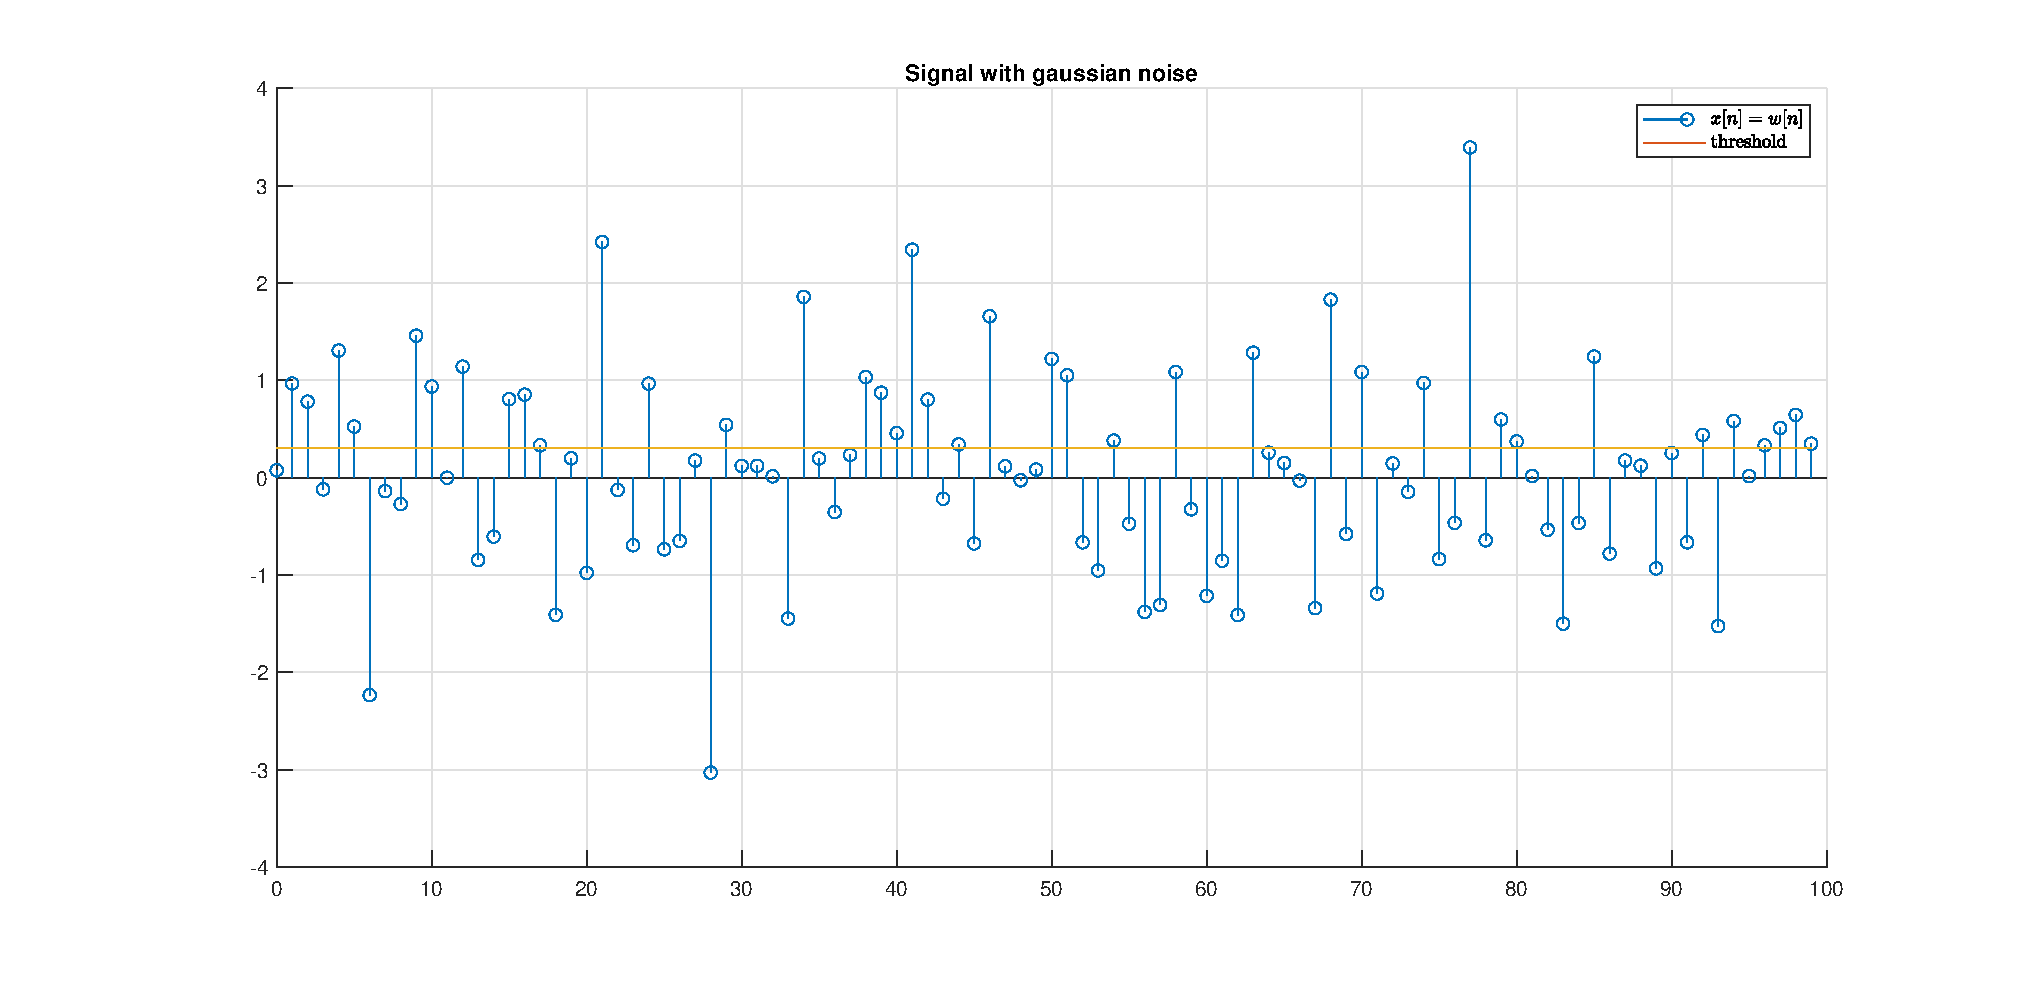
\includegraphics[width = \linewidth]{figures/gen_sign_noise.eps}
	\caption{100 samples from a gaussian distribution $\mathcal{N}(0,1)$}
	\label{fig:noise}
\end{figure}
From these 100 samples there are 39 samples that are above the set threshold meaning that from these 100 samples we will get 39 false positives/alarms which will alert the user that there is an object detected when there really is not. Our goal when solving detection problems is to develop a detector that from the samples can find a decision rule so that the number of false alarms is minimized but at the same time manages to detect correctly when there is an object present.\cite{Myrvoll2020}\\
\subsection{Neyman-Pearson detector}
The Neyman-Pearson detector utilizes the likelihood ratio test (LRT)
\begin{equation}
	L(\mathbf{x}) \triangleq \frac{p_1(\mathbf{x})}{p_0(\mathbf{x})} 
		\begin{cases}
			\geq \lambda \implies H_1
			< \lambda \implies H_0
		\end{cases} 
\end{equation}
where $p_1(x)$ and $p_0(x)$ is the point distribution functions or the likelihood functions of the distributions under $H_1$ and $H_0$ respectively.
With the Neyman-Pearson detector the threshold $\lambda$ is chosen to satisfy the constraint and to maximize the power such that
\begin{equation}
	P_{FA} = \alpha = \int_{L(\mathbf{x})>\lambda}p_0(\mathbf{x})d\mathbf{x}
\end{equation}
where $\alpha_0$ the tuning factor. This goes hand in hand with the detection rate of the detector as well since the Neyman-pearson lemma states that to increase the power of the likelihood ratio test, the false alarm rate is also increased. \todo{Mye dårlige formuleringer her. Må skrives om}
\begin{enumerate}[i]
	\item \underline{Inform} the reader that this chapter is a presentation of the theory needed to understand the task
	\item You may copy parts from lecture notes (but inform
	the reader that you have done this!). Also refer to
	books in former courses or other literature
	\begin{itemize}
		\item Always refer to the source and
		\item Use quotation marks when quoting (copying) 
	\end{itemize}
	\item Use figures if possible/natural!
\end{enumerate}
\section{The tasks}\label{sec:task}
The main problem that is going to be solved in this project is the detection problem
\begin{align}
\begin{split}
	H_0: x(n) & = w(n), n = 0, 1, \dots, N-1\\
	H_1: x(n) & = s(n) + w(n), n = 0, 1, \dots, N-1
\end{split}
\end{align}\label{eq:detection_problem}
where $s(n)$ is a waveform sequence of the PU and $w(n)$ is an additive white complex gaussian noise.
To construct the sequence $s(n)$, that is transmitted over the wireless channel, the modulation method orthogonal frequency-division multiplexing (OFDM) is used. Each information symbol $S(k)$, $k=0,1,\dots,N-1$ is allocated on each N carrier frequencies. The unique time-domain signal $s(n)$ corresponding to the sampled spectrum is obtained by inverse discrete fourier transform. Thus is the PUs time-domain signal given by:
\begin{equation}
	s(n) = \frac{1}{\sqrt{N}}\sum_{k=0}^{N-1}S(k)e^{\frac{j2\pi nk}{N}}, n = 0,1,\dots,N-1
\end{equation}
which we notice is a complex-valued quantity.

\subsection{Task 1: Model building}
Here the data $x[n]$ is generated, which can be used in our analysis to obtain a suitable detector. To generate $x[n]$ we need do to verify that the complex-valued time-domain OFDM signal sequence $s(n) = s_R(n)+js_I(n)$ is independent and identically distributed, in addition to verify that it is accurately modelled with a complex gaussian distribution.\\
Here the datasets T1 are used as the information symbol sent over. The two datasets contains samples that are taken from a standard normal Gaussian distribution and binary phase shift keying respectively.

\subsection{Task 2: One-sample detector}
In this task only a single sample is used to generate the NP-detector. That is there needs to be done calculations to retrieve the decision rule that decides for when to choose null hypothesis over the alternative hypothesis and vice versa.

\subsection{Task 3: Performance of the one-sample detector}
Here the datasets T3 are given and are to be used to verify that
\begin{align}
	H_0 &: \frac{2x_R^2(0)}{\sigma_w^2}+\frac{2x_I^2(0)}{\sigma_w^2}=\frac{2|x(0)|^2}{\sigma_w^2}\label{eq:chi_sq_h0}\\
	H_1 &: \frac{2x_R^2(0)}{\sigma_w^2+\sigma_s^2}+\frac{2x_I^2(0)}{\sigma_w^2+\sigma_s^2}=\frac{2|x(0)|^2}{\sigma_w^2+\sigma_s^2}\label{eq:chi_sq_h1}
\end{align}
are $\chi^2$-distributed with 2 degrees of freedom. Using this we can approximate that $\frac{2|x(0)|^2}{\sigma^2}$ has the point-distribution function $f(x) = \frac{1}{2}e^{-\frac{x}{2}}$ for $x>0$. Which is more manageable than the pdf for the complex gaussian so that it can be used to easily find the probability of detection and false alarm.

\subsection{Task 4: NP detector with data set of $K$ samples}
Here the one-sample detector derived in the previous tasks are expanded so it can be used when there are $K>1$ samples. Then the threshold $\lambda'$ is derived so that in this case probability of detection is maximized and probability of false alarm is less than a given limit $\alpha$.

\subsection{Task 5: Performance of the general NP detector}
First compute the distribution of the test statistic obtained in the previous task under hypothesis $H_0$ and $H_1$. Plot the receiving operating characteristics.

\subsection{Task 6: Approximate performance of the general NP detector}
Central limit theorem to approximate the characteristic test statistic as a gaussian random variable and compute the PDF of the test statistic. Plot $P_D$ and $P_{FA}$ as a function of the threshold.

\subsection{Task 7: Complexity of the detector}
Use approximation in task 6 and find an expression to compute the number of samples required to attain a given $P_{FA}$ and $P_D$.

\subsection{Task 8: Numerical experiments in PU detection}
Given a dataset of numerical experiment data, apply the NP detector to decide wether a PU is present or not. Discuss the results
\begin{enumerate}[i]
	\item Give a short description of all tasks and why are we doing these tasks
	\item Describe the task
\end{enumerate}
\section{Implementation and results}\label{sec:results}
\subsection{Task 1: Model development}
\todo{Legg til figurer og kommentarer for første oppgaven}
\subsection{Task 2: One-sample-detector}
In this task only one sample is used meaning that the detection problem is in this case:
\begin{align}
    H_0 &: x(0) = w(0)\nonumber\\
    H_1 &: x(0) = s(0)+w(0)\nonumber
\end{align}
It is given from the problem that $w\thicksim\mathbb{C}\mathcal{N}(0, \sigma_w^2)$ and $s\thicksim\mathbb{C}\mathcal{N}(\mu_s, \sigma_s^2)$ which means that under $H_0$, $x$ is from same distribution as $w$ and thus a complex gaussian with same mean and variance as $w$. Under $H_1$, which is a sum of two complex gaussian distribution, $x$ also is from a complex gaussian distribution, however the mean and variance needs to be calculated.
The mean of $x(0)$ under $H_1$ is\todo{Usikker på om det er vits med disse utregningene}
\begin{align}
    \mathbb{E}\{x(0)\} & = \mathbb{E}\{s(0)+w(0)\}\nonumber\\
    & = \mathbb{E}\{s(0)\} + \mathbb{E}\{w(0)\}\nonumber\\
    & = \mu_s + 0 = \mu_s\nonumber
\end{align} 
The variance of $x(0)$ under $H_1$ is
\begin{align}
    \mathrm{Var}\{x(0)\} & = \mathrm{Var}\{s(0)+w(0)\}\nonumber\\
    & = \mathrm{Var}\{s(0)\} + \mathrm{Var}\{w(0)\}\nonumber\\
    & = \sigma_s^2+\sigma_w^2\nonumber
\end{align}
Meaning that
\begin{align}
    p(x;H_0) & = p_0(x) = \frac{1}{\sigma_w^2\pi}e^{-\frac{|x|^2}{\sigma_w^2}}\\
    p(x;H_1) & = p_1(x) = \frac{1}{(\sigma_w^2+\sigma_s^2)\pi}e^{-\frac{|x-\mu_s|^2}{\sigma_s^2+\sigma_w^2}}
\end{align}
Setting up the LRT:
\begin{align}
    L(x) & = \frac{p_1(x(0))}{p_0(x(0))} = \frac{\frac{1}{(\sigma_w^2+\sigma_s^2)\pi}e^{-\frac{|x(0)-\mu_s|^2}{\sigma_s^2+\sigma_w^2}}}{\frac{1}{\sigma_w^2\pi}e^{-\frac{|x(0)|^2}{\sigma_w^2}}}\nonumber\\
    & = \frac{\sigma_w^2}{\sigma_w^2+\sigma_s^2}e^(-\frac{1}{\sigma_w^2+\sigma_s^2}|x(0)-\mu_s|^2+\frac{1}{\sigma_w^2}|x(0)|^2)\nonumber
\end{align}
Since it was shown in task 1 that $\mu_s \simeq 0$ this can be used to simplify the caluclations. The decision rule is to choose $H_1$ when $L(x) \geq \lambda$, since $L(x(0))$ is a monotonically increasing function then the inequality holds for $\ln L(x(0)) \geq \ln\lambda$.
\begin{align}
    \ln L(x(0)) = \ln (\sigma_w^2)-\ln (\sigma_w^2+\sigma_s^2)-\frac{1}{\sigma_w^2+\sigma_s^2}|x(0)|^2+\frac{1}{\sigma_w^2}|x(0)|^2 \geq \ln\lambda\nonumber\\
    (\frac{1}{\sigma_w^2}+\frac{1}{\sigma_s^2+\sigma_w^2})|x(0)|^2 \geq \ln\lambda-\ln (\frac{\sigma_w^2}{\sigma_w^2+\sigma_s^2})\nonumber\\
    |x(0)|^2 = x_R(0)^2+x_I(0)^2 \geq \frac{\sigma_w^2(\sigma_w^2+\sigma_s^2)}{\sigma_s^2}(\ln\lambda-\ln (\frac{\sigma_w^2}{\sigma_w^2+\sigma_s^2})) = \lambda'
\end{align}

\begin{enumerate}[i]
    \item What is this chapter about
    \item Matlab implementation
    \item Any specific Matlab m-commands used?
    \item A flow-diagram is recommended
    \item Results (use figures/tables if possible)
    \item Discussion of results
    \item Matlab code (documented) in appendix
\end{enumerate}
\section{Conclusion}\label{sec:conclusion}
This project focused on Spectrum Sensing in OFDM Cognitive Radios, which is an important problem in modern communication as the spectrum is a scarce resource. After modeling how the signal data was generated, a suitable detector for the binary hypothesis testing was implemented. This was a result of using well known statistical features of the Gamma and Gaussian distribution, as well as the Neyman-Person Lemma. After testing the performance of the one-sample-detector, a more generalized K-sample detector was implemented. This new NP detector for K samples was then approximated as a Gaussian random variable which showed to be quite accurate to the original gamma distribution. This detector based on K samples showed to be useful in the way that one could choose a $P_{D}$ and $P_{FA}$ only at the cost of more samples K. In the end, this whole detector was put to a test when a data set of 100 realizations of a signal from a PU was tested on the detector. As the result in task 8 have shown, the detector did very well, and detected the signal almost every time, however increasing K manually gave a detection rate of $100\%$.\\
The project has been very educational and it has been specifically interesting to see how probability distributions are used in modern communications systems for hypothesis testing. With an increasing number of communication devices this problem is highly relevant.




% References
\newpage
\addcontentsline{toc}{section}{References}
\printbibliography{}
\label{sec:bibliography}

% appendix of matlab codes
\addcontentsline{toc}{section}{Appendix} % Remove this if you don't want the appendix included in the table of contents.
\appendix
\section{MATLAB code}
\subsection{Problem 1}\label{sec:prob1}
\lstinputlisting{code/problem1.m}
\subsection{Problem 3}\label{sec:prob3}
\lstinputlisting{code/problem3.m}
\subsection{Problem 5}\label{sec:prob5}
\lstinputlisting{code/problem5.m}
\subsection{Problem 6}\label{sec:prob6}
\lstinputlisting{code/problem6.m}
\subsection{Problem 8}\label{sec:prob8}
\lstinputlisting{code/problem8.m}
% \input simply inserts the contents of the file, while \include forces a \newpage.\text{Null hypothesis} H_0 & : x[n] \thicksim P_0\nonumber\\
% See \input vs. \include: http://tex.stackexchange.com/questions/246/when-should-i-use-input-vs-include

\end{document}
